%problem 6 needs a picture
%13 14


3.1 对Markov链$X_n, n \geqslant 0$, 试证条件
	\[
	P\{X_{n+1} = j | X_0 = i_0, \cdots , X_{n-1} = i_{n-1}, X_n = i\} = P\{X_{n+1} = j | X_n = i\}
	\]
	等价于对所有时刻$n, m$及所有状态$i_0, \cdots, i_n, j_1, \cdots, j_m$有
	\[
	\begin{split}
	& \quad P\{X_{n+1} = j_1, \cdots, X_{n+m} = j_m | X_0 = i_0, \cdots, X_n = i\}\\
	& = P\{X_{n+1} = j_1, \cdots, X_{n+m} = j_m | X_n = i_n\}.
	\end{split}
	\]
证:$\Leftarrow $只需令$m=1$\\
	$\Rightarrow $由$P_{27}(3.4)$可知\\
	\[
	\begin{split}
	& \quad P\{X_{n+1} = j_1, \cdots, X_{n+m} = j_m | X_0 = i_0, \cdots, X_n = i_n\}\\
	& = P\{X_{n+1} = j_1, \cdots, X_{n+m} = j_m , X_0 = i_0, \cdots, X_n = i_n\} / P\{X_0 = i_0, \cdots, X_n = i_n\}\\
	& = P\{X_0 = i_0\} \cdot P_{j_1j_2} \cdots P_{j_{m-1}j_m} P_{i_0i_1} \cdots P_{i_1j_1} / [P\{X_0 = i_0\} \cdot P_{i_0i_1} \cdots P_{i_{n-1}i_n}\\
	& = P\{X_n = i\} \cdot P_{j_1j_2} \cdots P_{j_{m-1}j_m} P_{i_nj_1} / P\{X_n = i_n\}\\
	& = P\{X_{n+1} = j_1, \cdots, X_{n+m} = j_m | X_n = i_n\}\\
	\end{split}
	\]


3.2 考虑状态 $ 0,1,2 $ 上的一个Markov链$X_n, n \geqslant 0$, 它有转移概率矩阵
	\[
	P = \begin{pmatrix}
	0.1 & 0.2 & 0.7 \\
	0.9 & 0.1 & 0 \\
	0.1 & 0.8 & 0.1 
	\end{pmatrix} ,
	\]
	初始分布为$p_0 = 0.3, p_1 = 0.4, p_2 = 0.3$, 试求概率$P\{X_0 = 0, X_1 = 1, X_2 = 2\}$.\\
解:
	\[
	P\{X_0 = 0, X_1 = 1, X_2 = 2\} = p_0P_{01}P_{12} = 0.3 \times 0.1 \times 0 = 0
	\]


3.3 信号传送问题. 信号只有 $0,1$ 两种, 分为多个阶段传输. 在每一步上出错的概率为 $\alpha$ . $X_0 = 0$ 是送出的信号, 而 $X_n$ 是在第 $n$ 步接收到的信号. 假定$X_n$为一Markov链, 它有转移概率矩阵 $P_{00} = P_{11} = 1 - \alpha , P_{01} = P_{10} = \alpha, 0 < \alpha < 1$. 试求\\
(a) 两步均不出错的概率$P\{X_0 = 0, X_1 = 0, X_2 = 0\}$;\\
(b) 两步传送后收到正确信号的概率;\\
(c) 五步之后传送无误的概率$P\{X_5 = 0 | X_0 = 0\}$.\\
解:
(a) $P\{X_0 = 0, X_1 = 0, X_2 = 0\} = p_0P_{00}P_{00} = 1 \cdot (1-\alpha) \cdot (1-\alpha) = (1-\alpha)^2$;\\
(b) $P = p_0P_{00}P_{00} + p_0P_{01}P_{10} = (1-\alpha)^2 + {\alpha}^2 = 2{\alpha}^2 - 2\alpha + 1$\\
(c) 转移概率矩阵
	$
	P = \begin{pmatrix} \frac{\sqrt{2}}{2} & \frac{\sqrt{2}}{2}\\ \frac{\sqrt{2}}{2} & -\frac{\sqrt{2}}{2} \end{pmatrix}^{-1}
	\begin{pmatrix} 1 & 0 \\ 0 & 1-2\alpha \end{pmatrix}
	\begin{pmatrix} \frac{\sqrt{2}}{2} & \frac{\sqrt{2}}{2}\\ \frac{\sqrt{2}}{2} & -\frac{\sqrt{2}}{2} \end{pmatrix}
	$\\
	\[
	\begin{aligned}
	\therefore P^{(5)} & =  
		\begin{pmatrix} \frac{\sqrt{2}}{2} & \frac{\sqrt{2}}{2}\\ \frac{\sqrt{2}}{2} & -\frac{\sqrt{2}}{2} \end{pmatrix}^{-1}
		\begin{pmatrix} 1 & 0 \\ 0 & (1-2\alpha)^5 \end{pmatrix}
		\begin{pmatrix} \frac{\sqrt{2}}{2} & \frac{\sqrt{2}}{2}\\ \frac{\sqrt{2}}{2} & -\frac{\sqrt{2}}{2} \end{pmatrix}\\
					& = \begin{pmatrix}
					\frac{1+(1-2\alpha)^5}{2} & \frac{1-(1-2\alpha)^5}{2}\\ \frac{1-(1-2\alpha)^5}{2}& \frac{1+(1-2\alpha)^5}{2}
					\end{pmatrix}
	\end{aligned}
	\]
	$\therefore P\{ X_5 = 0 | X_0 = 0\} = p_0 \cdot \frac{1+(1-2\alpha)^5}{2} = \frac{1+(1-2\alpha)^5}{2}$\\


3.4 $A, B$ 两罐总共装各 $N$ 个球. 作如下实验:在时刻 $n$ 先 $n$ 个球中等概率地任取一球. 然后从 $A, B$ 两罐中任选一个, 选中 $A$ 的概率为 $p$, 选中 $B$ 的概率为 $q$. 之后再将选出的球放入选好的罐中. 设 $X_n$ 为每次试验时 $A$ 罐中的球数. 试求此Markov过程的转移概率矩阵.\\
解:
\[
P_{ij} = 
\begin{cases}
p \cdot \frac{i}{N} + q \cdot \frac{N-i}{N} & , j = i\\
q \cdot \frac{i}{N} & , j = i-1(i=1,2,\cdots ,N)\\
p \cdot \frac{N-i}{N} & , j = i+1(i=0,1,\cdots ,N-1)\\
0 & , \text{其他}
\end{cases}
\]
其转移概率矩阵为
\[
P = \frac{1}{N} 
\begin{pmatrix}
qN & pN & 0 & \cdots & 0 & 0 & 0 \\
q & q(N-1)+p & p(N-1) & \cdots & 0 & 0 & 0 \\
0 & 2q & q(N-2)+2p & \cdots & 0 & 0 & 0\\
\vdots & \vdots & \vdots & \ddots & \vdots & \vdots & \vdots \\
0 & 0 & 0 & \cdots & 2q+p(N-2) & 2p & 0\\
0 & 0 & 0 & \cdots & q(N-1) & q+p(N-1) & p\\
0 & 0 & 0 & \cdots & 0 & qN & pN
\end{pmatrix}
\]


3.5 重复掷币一直到连续出现两次正面为止. 假定钱币是均匀的, 试引入以连续出现次数为状态空间的Markov链, 并求出平均需要掷多少次试验才可以结束.\\
解:记$X_n$为第$n$次掷币后连续出现的正面次数, 则$\{X_n, n \geqslant 0 \}$为一$M.C.$\\
其转移概率矩阵为$P = \bordermatrix{
				~ & 0 & 1 & 2 \cr
				0 & \frac{1}{2} & \frac{1}{2} & 0 \cr
				1 & \frac{1}{2} & 0 & \frac{1}{2} \cr
				2 & 0 & 0 & 1 
				}$\\
\[
\begin{split}
\therefore & \quad E(T | X_0 = 0)\\
		& = \sum^2_{k=0}E(T|X_0 = 0, X_1 = k)\cdot P(X_1 = k | X_0 = 0)\\
		& = \sum^2_{k=0}E(T|X_1 = k)\cdot P(X_1 = k | X_0 = 0)\\
		& = (1+v)\cdot \frac{1}{2} + E(T| X_1 = 1) \cdot \frac{1}{2}\\
\text{及}& \quad E(T | X_1 = 1)\\
		& = \sum^2_{k=0}E(T|X_1 = 1, X_2 = k)\cdot P(X_2 = k | X_1 = 1)\\
		& = \sum^2_{k=0}E(T|X_2 = k)\cdot P(X_2 = k | X_1 = 1)\\
		& = (2+v)\cdot \frac{1}{2} + 0 + \frac{1}{2} \times 2
\end{split}
\]
解得$E(T | X_0 = 0) = 6$, 平均需掷$6$次. \\


3.6 迷宫问题. 将小家鼠放入迷宫内作动物的学习试验, 如下图所示. 在迷宫的第$7$号小格内放有美味食物而第$8$号小格内则是电击捕鼠装置. 假定当家鼠位于某格时有$k$个出口可以离去, 则它总是随机地选择一个, 概率为$1/k$. 并假定每一次家鼠只能跑到相邻的小格去. 令过程$X_n$为家鼠在时刻$n$时所在小格的号码, 试写出这一Markov过程的转移概率阵, 并求出家鼠在遭到电击前能找到食物的概率.\\
\begin{figure}[htbp]
	\centering
	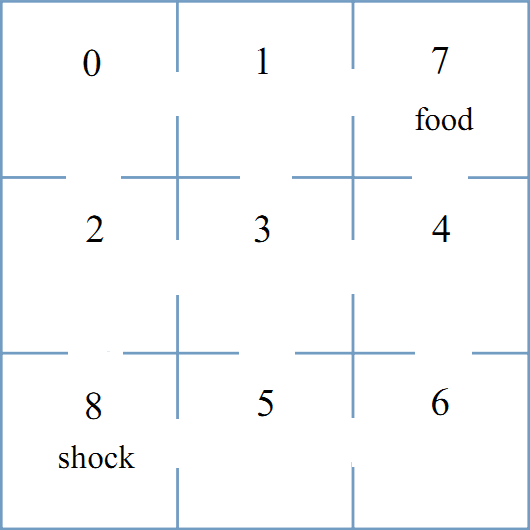
\includegraphics[width=0.3\textwidth]{../resource/maze.png}
\end{figure}\\
解:\\
\[
P = 
\bordermatrix{
	~ & 0 & 1 & 2 & 3 & 4 & 5 & 6 & 7 & 8 \cr
	0 & 0 & \frac{1}{2} & \frac{1}{2} & 0 & 0 & 0 & 0 & 0 & 0 \cr
	1 & \frac{1}{3} & 0 & 0 & \frac{1}{3} & 0 & 0 & 0 & \frac{1}{3} & 0 \cr
	2 & \frac{1}{3} & 0 & 0 & \frac{1}{3} & 0 & 0 & 0 & 0 & \frac{1}{3}\cr
	3 & 0 & \frac{1}{4} & \frac{1}{4} & 0 & \frac{1}{4} & \frac{1}{4} & 0 & 0 & 0 \cr
	4 & 0 & 0 & 0 & \frac{1}{3} & 0 & 0 &\frac{1}{3} & \frac{1}{3} & 0 \cr
	5 & 0 & 0 & 0 & \frac{1}{3} & 0 & 0 &\frac{1}{3} & 0 & \frac{1}{3} \cr
	6 & 0 & 0 & 0 & 0 & \frac{1}{2} & \frac{1}{2} & 0 & 0 & 0 \cr
	7 & 0 & 0 & 0 & 0 & 0 & 0 & 0 & 1 & 0 \cr
	8 & 0 & 0 & 0 & 0 & 0 & 0 & 0 & 0 & 1 \cr
}
\]
设$u_k$为家鼠从$k$出发在遭到电击前能找到食物的概率, 显然$u_7 = 1, u_8 = 0$,\\
设$T$为进入吸收态时刻, 则当$0 \leqslant k \leqslant 6$时, 
\begin{align*}
u_k & = P\{X_T = 7 | X_0 = k\}\\
	& = \sum^8_{i=0}P\{X_T = 7, X_1 = i | X_0 = k\}\\
	& = \sum^8_{i=0}P\{X_T = 7, X_1 = i\} P\{X_1 = i | X_0 = k\}
\end{align*}
\[
\therefore
\begin{cases}
u_0 = \frac{1}{2}(u_1+u_2)\\
u_1 = \frac{1}{3}(u_0+u_3+u_7)\\
u_2 = \frac{1}{3}(u_0+u_3+u_8)\\
u_3 = \frac{1}{4}(u_1+u_2+u_4+u_5)\\
u_4 = \frac{1}{3}(u_3+u_6+u_7)\\
u_5 = \frac{1}{3}(u_3+u_6+u_8)\\
u_6 = \frac{1}{2}(u_4+u_5)\\
u_7 = 1\\
u_8 = 0
\end{cases}
\Rightarrow
\begin{cases}
u_0 = \frac{1}{2}\\
u_1 = \frac{2}{3}\\
u_2 = \frac{1}{3}\\
u_3 = \frac{1}{2}\\
u_4 = \frac{2}{3}\\
u_5 = \frac{1}{3}\\
u_6 = \frac{1}{2}\\
u_7 = 1\\
u_8 = 0
\end{cases}
\]


3.7 记$Z_i, i = 1, 2, \cdots$ 为一串独立同分布的离散随机变量. $P\{Z_1 = k\} = p_k \geqslant 0, k = 0,1,2,\cdots, \sum\limits^\infty_{k=0} = 1$. 记$X_n = Z_n, n = 1, 2, \cdots$. 试求过程$X_n$的转移概率矩阵.\\
解:
$\because P\{X_{n+1} = i_{n+1} | X_1 = i_1, \cdots , X_n = i_n\} = P\{X_{n+1} = i_{n+1}\}$\\
$P\{X_{n+1} = i_{n+1} | X_n = i_n\} = P\{X_{n+1} = i_{n+1}\}$\\
$\therefore P\{X_{n+1} = i_{n+1} | X_1 = i_1, \cdots , X_n = i_n\} = P\{X_{n+1} = i_{n+1} | X_n = i_n\}$\\
$\therefore \{X_n\}$是一$M.C.$ ~~~其转移概率矩阵为
\[
P = 
\begin{pmatrix}
p_0 & p_1 & p_2 & \cdots \\
p_0 & p_1 & p_2 & \cdots \\
p_0 & p_1 & p_2 & \cdots \\
\vdots & \vdots & \vdots & \ddots
\end{pmatrix}
\]


3.8 对第7题中的$Z_i$, 令$X_n = \max \{Z_1, \cdots , Z_n\}, n = 1, 2, \cdots$, 并约定$X_0 = 0$. $X_n$是否为Markov链? 如果是, 其转移概率阵是什么?\\
解:\\
\begin{align*}
X_{n+1} & = \max \{Z_1, \cdots, Z_n, Z_{n+1}\}\\
		& = \max \{\max\{Z_1, \cdots, Z_n\}, Z_{n+1}\}\\
		& = \max \{X_n, Z_{n+1}\}
\end{align*}
$\therefore \{X_n\}$是$M.C.$\\
\[
P_{ij} = 
\begin{cases}
0 & , j < i\\
p_j & , j > i\\
\sum\limits^i_{k=0}p_k & , j = i\\
0 & , \text{其他}
\end{cases}
\]
其转移概率矩阵为
\[
P = 
\begin{pmatrix}
p_0 & p_1 & p_2 & \cdots \\
0 & p_0+p_1 & p_2 & \cdots \\
0 & 0 & p_0+p_1+p_2 & \cdots \\
\vdots & \vdots & \vdots & \ddots
\end{pmatrix}
\]


3.9 设$f^{(n)}_{ij}$表示从$i$出发在$n$步转移时首次到达$j$的概率, 试证明
\[
P^{(n)}_{ij} = \sum^n_{k=0}f^{(k)}_{ij}P^{(n-k)}_{jj}.
\]
证:
设$T_j = \min \{n: n \geqslant 0 \text{且} X_n = j\}$\\
\[
\begin{split}
\therefore P^{(n)}_{ij} & = P\{X_n = j | X_0 = i\}\\
				& = \sum^n_{k=0}P\{X_n = j, T_j = k | X_0 = i\}\\
				& = \sum^n_{k=0}P\{T_j = k | X_0 = i\}P^{(n-k)}_{jj}\\
				& = \sum^n_{k=0}P\{X_k = j, X_s\neq j(s = 0,1,\cdots, k-1) | X_0 = i\}P^{(n-k)}_{jj}\\
				& = \sum^n_{k=0}f^{(k)}_{ij} P^{(n-k)}_{jj}
\end{split}
\]


3.10 对第7题中的$Z_i$, 若定义$X_n = \sum\limits^n_{i=1}Z_i, n = 1, 2, \cdots, X_0 = 0$, 试证$X_n$为Markov链. 并求其转移概率矩阵.\\
证:
对$n \geqslant 0$有\\
\[
\begin{split}
& \quad P\{X_{n+1} = i_{n+1} | X_0 = i_0, \cdots, X_n = i_n\}~~~~(i_0 = 0)\\
& = P\{Z_{n+1} = i_{n+1} - i_n | X_0 = i_0, \cdots, X_n = i_n\}\\
& = P\{Z_{n+1} = i_{n+1} - i_n\}\\
& = 
\begin{cases}
P_{i_{n+1}-i_n} &, i_{n+1} - i_n = 0,1,2,\cdots\\
0 &, ow
\end{cases}
\end{split}
\]
\[
\begin{split}
& \quad P\{X_{n+1} = i_{n+1} | X_n = i_n\}\\
& = P\{X_{n} + Z_{n+1} = i_{n+1} | X_n = i_n\}\\
& = P\{Z_{n+1} = i_{n+1} - i_n\}\\
\end{split}
\]
$\therefore X_n $是$M.C.$\\
\[
P = 
\begin{pmatrix}
p_0 & p_1 & p_2 & \cdots \\
0	& p_0 & p_1 & \cdots \\
0	& 0	  & p_0 & \cdots \\
\vdots & \vdots & \vdots & \ddots
\end{pmatrix}
\]


3.11 一Markov链有状态$0,1,2,3$和转移概率矩阵
\[
P = 
\begin{pmatrix}
0 & \frac{1}{2} & 0 & \frac{1}{2}\\
0 & 0 & 1 & 0\\
0 & 0 & 0 & 1\\
\frac{1}{2} & 0 & 0 & \frac{1}{2}\\
\end{pmatrix}
\]
试求$f^{(n)}_{00}, n = 1,2,3,4,5,\cdots, $ 其中$f^{(n)}_{00}$由
\[
P\{X_n = i, X_k \neq i, k = 1, \cdots, n-1 | X_0 = i\}
\]
定义.\\
解:$f^{(1)}_{00} = P_{00} = 0, f^{(2)}_{00} = \begin{pmatrix}\frac{1}{2} & 0 & \frac{1}{2}\end{pmatrix}\begin{pmatrix}0 & 0 & \frac{1}{2}\end{pmatrix}^T = \frac{1}{4} $\\
对$n \geqslant 2$有
\[
f^{(n)}_{00} = \begin{pmatrix}\frac{1}{2} & 0 & \frac{1}{2}\end{pmatrix}
	\begin{pmatrix}
	0 & 1 & 0 \\
	0 & 0 & 1 \\
	0 & 0 & \frac{1}{2}\\
	\end{pmatrix}^{n-2}
	\begin{pmatrix}0 \\ 0 \\ \frac{1}{2}\end{pmatrix}
\]
当$n=3$时, $f^{(3)}_{00} = \frac{1}{8}$\\
当$n \geqslant 4$时, 
\[
f^{(n)}_{00} = \begin{pmatrix}\frac{1}{2} & 0 & \frac{1}{2}\end{pmatrix}
	\begin{pmatrix}
	0 & 0 & \frac{1}{2^{n-2}}\\
	0 & 0 & \frac{1}{2^{n-1}}\\
	0 & 0 & \frac{1}{2^{n-1}}\\
	\end{pmatrix}
	\begin{pmatrix}0 \\ 0 \\ \frac{1}{2}\end{pmatrix}
	= \frac{1}{2^n} + \frac{1}{2^{n+2}}
\]


3.12 在成败型的重复试验中, 每次试验结果为成功(S)或失败(F). 同一结果相继出现称为一个游程(run), 比如一结果$FSSFFFSF$中共有两个成功游程, 三个失败游程. 设成功概率为$p$, 失败概率为$q = 1 - p$. 记$X_n$为第$n$次试验后成功游程的长度(若第$n$次试验, 则$X_n = 0$). 试证$\{X_n, n = 1,2,\cdots\}$为一Markov链, 并确定其转移概率阵. 记$T$为返回状态$0$的时间, 试求$T$的分布及均值. 并由此对这一Markov链的状态进行分类.\\
证:$
	X_{n+1} = \begin{cases}
				X_{n+1} & , \text{第n+1次试验成功}\\
				0 & , \text{第n+1次试验失败}\\
				\end{cases}
	$\\
	$\therefore \{X_n\}$是$M.C.$\\
	$P(X_{n+1} = j | X_n = i) = \begin{cases}
		p & , j = i + 1\\
		q & , j = 0\\
		\end{cases}$
	\[
	P = 
	\bordermatrix{
		~ & 0 & 1 & 2 & 3 & \cdots \cr
		0 & q & p & 0 & 0 & \cdots \cr
		1 & q & 0 & p & 0 & \cdots \cr
		2 & q & 0 & 0 & p & \cdots \cr
		\vdots & \vdots & \vdots & \vdots & \vdots & \ddots \cr
	}
	\]
	\[
	\begin{split}
	&T = \min \{n : X_n = 0, X_s \neq 0(s = 1,2,\cdots, n-1)\}\\
	&P(T = k) = p^{k-1}q~~~~k = 1, 2, \cdots\\
	&\E T = \sum^{+\infty}_{k=1}p^{k-1}qk\\
	&\therefore p\E T = \sum^{+\infty}_{k=1}p^kqk\\
	&\therefore (1-p)\E T = q\E T = q + pq + p^2q + \cdots = \frac{q}{1-p} = 1\\
	&\therefore \E T = \frac{1}{q}\\
	\end{split}
	\]
	\begin{figure}[htbp]
		\centering
		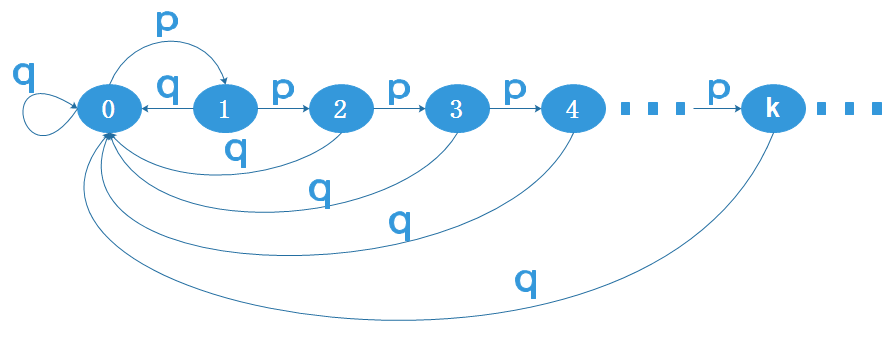
\includegraphics[width=0.8\textwidth]{../resource/sp3_12.png}
	\end{figure}\\
	所有状态互通, 为一类\\



3.13 试证各方向游动的概率相等的对称随机游动在二维时是常返的%, 而在三维时却是瞬过的.\\
\\%应说清这个随机过程的定义
证:为使n步游动后回到原位置, 向左移动的步数应等于向右移动的步数, 向上移动的步数应等于向下移动的步数, $\therefore P^{(2k+1)}_{00} = 0, k = 0, 1, 2,\cdots$\\
再考虑2k步的情况, \\
\[
\begin{split}
P^{(2k)}_{00} & = \sum^k_{k_1 = 0}C^{k-k_1}_{2k-2k_1}C^{k_1}_{2k_1}C^{2k_1}_{2k}\left(\frac{1}{4}\right)^{2k}\\
			& = \sum^k_{k_1 = 0}\frac{(2k)!}{(k!)^2}\left(C^{k_1}_k\right)^2\left(\frac{1}{2^{2k}}\right)^2\\
            & = \frac{(2k)!}{(k!)^2}\left(\frac{1}{2^{2k}}\right)^2\sum^k_{k_1 = 0}C^{k_1}_kC^{k-k_1}_k\\
            & = \frac{(2k)!}{(k!)^2}\left(\frac{1}{2^{2k}}\right)^2C^{k}_{2k}\\
            & = \left(\frac{(2k)!}{(k!)^2} \cdot \frac{1}{2^{2k}}\right)^2
\end{split}
\]


当$n$充分大时, 由Stiring公式
\[
P^{(2k)}_{00} \sim \left(\frac{(2k)^{2k+\frac{1}{2}} e^{-2k} \sqrt{2\pi}}{(k^{k+\frac{1}{2}} e^{-k} \sqrt{2\pi})^2} \cdot \frac{1}{2^{2k}}\right)^2 = \frac{1}{\pi k}
\]
$\therefore \sum\limits^{+\infty}_{n=1}P^{(n)}_{ii} = +\infty$   (i代表任一格点)\\
$\therefore $二维对称随机游动是常返的\\


3.14 某厂对该厂生产的同类产品的三种型号调查顾客的消费习惯. 并把它们归结为Markov链模型. 记顾客消费习惯在 $A, B, C $ 三种型号间的转移概率矩阵分别为下列四种. 请依这些转移阵所提供的信息对厂家提出关于 $A, B$ 两种型号的咨询意见.\\
\[
\begin{split}
&(1)\begin{pmatrix}
	1 & 0 & 0\\
	0 & 1 & 0\\
	0 & 0 & 0\\
	\end{pmatrix},~~~~~~~~
(2)\begin{pmatrix}
	0 & \frac{1}{2} & \frac{1}{2}\\
	\frac{1}{2} & 0 & \frac{1}{2}\\
	\frac{1}{2} & \frac{1}{2} & 0\\
	\end{pmatrix},\\
&(3)\begin{pmatrix}
	\frac{1}{2} & 0 & \frac{1}{2}\\
	\frac{1}{3} & \frac{1}{3} & \frac{1}{3}\\
	\frac{1}{2} & 0 & \frac{1}{2}\\
	\end{pmatrix},~~~~~~~~
(4)\begin{pmatrix}
	0 & 1 & 0\\
	0 & 0 & 1\\
	1 & 0 & 0\\
	\end{pmatrix}.
\end{split}
\]
解:\\
(1)不是概率转移矩阵, 第三行行和不为$1$.\\
(2)
\[
P^2 = 
\begin{pmatrix}
0 & \frac{1}{2} & \frac{1}{2}\\
\frac{1}{2} & 0 & \frac{1}{2}\\
\frac{1}{2} & \frac{1}{2} & 0\\
\end{pmatrix}^2
=
\begin{pmatrix}
\frac{1}{2} & \frac{1}{4} & \frac{1}{4}\\
\frac{1}{4} & \frac{1}{2} & \frac{1}{4}\\
\frac{1}{4} & \frac{1}{4} & \frac{1}{2}\\
\end{pmatrix}
\]
$\therefore A,B,C$三状态互通, 所有状态可遍历.\\
设$(\pi_A,\pi_B,\pi_C)$为经过长时间后三个产品的市场占有额,则
\[
\begin{cases}
(\pi_A,\pi_B,\pi_C)
\begin{pmatrix}
0 & \frac{1}{2} & \frac{1}{2}\\
\frac{1}{2} & 0 & \frac{1}{2}\\
\frac{1}{2} & \frac{1}{2} & 0\\
\end{pmatrix}
=
(\pi_A,\pi_B,\pi_C)\\
\pi_A+\pi_B+\pi_C = 1
\end{cases}
\Rightarrow~~
\pi_A = \pi_B = \pi_C = 1
\]
$\therefore$三个品牌竞争力差不多, 可以都生产.\\
(3)由归纳法可知
\[
P^n=
\begin{pmatrix}
\frac{1}{2} & 0 & \frac{1}{2}\\
\frac{1}{2}\big(1-\frac{1}{3^n}\big) & \frac{1}{3^n} & \frac{1}{2}\big(1-\frac{1}{3^n}\big)\\
\frac{1}{2} & 0 & \frac{1}{2}\\
\end{pmatrix}
\]
可见
\[
\pi_B = \lim_{n\rightarrow} \Big(\frac{1}{3}\Big)^n = 0,
\]
\[
\begin{cases}
(\pi_A, \pi_C)\cdot 
	\begin{pmatrix}
	\frac{1}{2} & \frac{1}{2}\\
	\frac{1}{2} & \frac{1}{2}\\
	\end{pmatrix}	
=
(\pi_A, \pi_C)\\
\pi_A + \pi_C = 1
\end{cases}
\Rightarrow~~
\pi_A = \pi_C = \frac{1}{2}
\]
$\therefore B$将逐渐淡出市场, 建议停止生产$B$, 扩大对$A$的生产.\\
(4)
\begin{figure}[htbp]
		\centering
		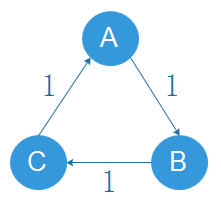
\includegraphics[width=0.2\textwidth]{../resource/sp3_14_4.png}
\end{figure}\\
$\therefore A,B,C$三状态互通, 所有状态可遍历.\\
\[
\begin{cases}
(\pi_A,\pi_B,\pi_C)
\begin{pmatrix}
0 & 1 & 0\\
0 & 0 & 1\\
1 & 0 & 0\\
\end{pmatrix}
=
(\pi_A,\pi_B,\pi_C)\\
\pi_A+\pi_B+\pi_C = 1
\end{cases}
\Rightarrow~~
\pi_A = \pi_B = \pi_C = \frac{1}{3}
\]
$\therefore A,B,C$市场占有率相同, 可维持现状.\\


3.15 考虑一有限状态的Markov链. 试证明\\
(a)至少有一个状态是常返的,\\
(b)任何常返状态必定是正常返的.\\
证:
(a)反设所有状态均为瞬过或零常返(加强结论),则对$\forall i \in S$, 有
	\[
	\lim_{n\rightarrow +\infty} P^{(n)}_{ii} = 0~~~~~~~~(*)
	\]
	考虑$P^{(n)}_{ij} = \sum\limits^{+\infty}_{k=1} f^{(k)}_{ij} P^{(n-k)}_{jj}$, 则有
	\[
	\sum^\ell_{k=1} f{(k)}_{ij} P^{(n-k)}_{jj} \leqslant P^{(n)}_{ij} \leqslant \sum^\ell_{k=1} f^{(k)}_{ij} P^{(n-k)}_{jj} + \sum^{+\infty}_{k=l} f^{(k)}_{ij}~~~~~~~(**)
	\]
	固定$\ell$, 令$n \rightarrow +\infty$, 则由$(*)$得
	\[
	0 \leqslant \lim_{n\rightarrow +\infty} P^{(n)}_{ij} \leqslant 0 + \sum^{+\infty}_{k=\ell} f^{(k)}_{ij}~~~~~~~(***)
	\]
	在$(***)$中令$\ell \rightarrow +\infty$, 由于$\sum\limits^{+\infty}_{k=1} f^{(k)}_{ij} \leqslant 1$收敛\\
	\[
	\therefore \lim_{n\rightarrow +\infty} P^{(n)}_{ij} = 0 ~~~~~~~~(*4)
	\]
	若此有限状态$M.C.$有$N$个状态, 则
	\[
	\sum^{N}_{j=1} P^{(n)}_{ij} = 1~~~~~~~(*5)
	\]
	$(*5)$中令$n\rightarrow +\infty$, 由$(*4)$得$0=1$, 矛盾\\
	$\therefore$至少有一个状态是(正)常返的\\
(b)若存在零常返状态$i$, 可构造$C(i) = \{j|i\leftrightarrow j\}$, 
	则$C(i)$为原$M.C.$的一不可约子$M.C.$(有限状态), 
	于是$C(i)$中所有状态均为零常返, 与有限状态$M.C.$至少有一个正常返状态矛盾, $\therefore$任何常返状态均为正常返


3.16 考虑一生长与灾害模型. 这类Markov链有状态 $0,1,2,\cdots,$ 当过程处于状态$i$时它既可能以概率$p_i$转移到$i+1$(生长)也能以概率$q_i = 1 - p_i$ 落回到状态$0$(灾害). 而从状态“0”又必然“无中”生有. 即$P_{01} \equiv 1$.\\
(a)试证所有状态为常返的条件是
\[
\lim_{n \rightarrow \infty}(p_1p_2p_3\cdots p_n) = 0.
\]
(b)若此链为常返, 试求其为零常返的条件.\\
证:\\
(a)其概率转移阵为
\[
P = 
\bordermatrix{
	~ & 0   & 1 & 2   & 3   & \cdots \cr
	0 & 0   & 1 & 0   & 0   & \cdots \cr
	1 & q_1 & 0 & p_1 & 0   & ~ \cr
	2 & q_2 & 0 & 0   & p_2 & ~ \cr
	3 & q_3 & 0 & 0   & 0 ~ \cr
	\vdots & \vdots & ~ & ~ & ~ & \ddots \cr
}
\]
易知此M.C.是不可约的, $\therefore$只需证状态$0$常返$\Leftrightarrow~\lim_{n\rightarrow +\infty}p_1p_2\cdots p_n = 0$\\
显然$f^{(0)}_{00} = f^{(1)}_{00} = 0, f^{(2)}_{00} = q_1$
\[
\begin{split}
f^{(n)}_{00} & = 
\begin{pmatrix}
1 & 0 & 0 & \cdots
\end{pmatrix}
\begin{pmatrix}
0 & p_1 & 0 & 0 & \cdots\\
0 & 0 & p_2 & 0 & \cdots\\
0 & 0 & 0 & p_3 & \cdots\\
\vdots & \vdots & \vdots & \vdots & \ddots\\
\end{pmatrix}^{n-2}
\begin{pmatrix}
q_1\\
q_2\\
q_3\\
\vdots
\end{pmatrix}\\
& = AB^{n-2}C^T, ~~(n\geqslant 3)
\end{split}
\]
易知
\[
B^{n-2} = 
\begin{pmatrix}
\underbrace{\begin{matrix}0 & \cdots & 0\end{matrix}}_{n-2\text{个}} & p_1\cdots p_{n-2} & 0 & \cdots \\
\underbrace{\begin{matrix}0 & \cdots & 0\end{matrix}}_{n-2\text{个}} & 0 & p_2\cdots p_{n-2} & \cdots \\
\vdots & \vdots & \vdots & \ddots\\
\end{pmatrix}
\]
\[
\therefore f^{(n)}_{00} = (\,\overbrace{0~\cdots~0}^{n-2\text{个}}~~p_1\cdots p_{n-2}~~0~~0~~\cdots)(q_1~~q_2~~\cdots)^T = p_1\cdots p_{n-2}q_{n-1}
\]
\[
\begin{split}
\therefore f_{00} & = q_1 + \sum^{+\infty}_{n=3}p_1\cdots p_{n-2}q_{n-1}\\
				& = 1 - p_1 + \sum^{+\infty}_{n=3}(p_1\cdots p_{n-2} - p_1\cdots p_{n-2}p_{n-1})\\
				& = 1 - \lim_{n\rightarrow +\infty}p_1p_2\cdots p_n\\
\end{split}
\]
而状态$0$常返$\Leftrightarrow f_{00} = 1 \Leftrightarrow \lim\limits_{n\rightarrow +\infty}p_1p_2\cdots p_n = 0$.\\
(b)只需考虑状态$0$, 
\[
\begin{split}
\mu_0 & = \sum^{+\infty}_{n=0}nf^{(n)}_{00}\\
	& = 2(1-p_1)+\sum^{+\infty}_{n=3}n(p_1\cdots p_{n-2} - p_1\cdots p_{n-1})\\
	& = 2 + p_1 + p_1p_2 + p_1p_2p_3 + \cdots
\end{split}
\]
若为零常返, 则$\mu_0 = +\infty \Leftrightarrow $级数$\sum\limits^{+\infty}_{n=1}p_1\cdots p_n$发散(且通项趋于$0$)


3.17 试计算转移概率阵
\[
P =
\begin{pmatrix}
	\frac{1}{2} & \frac{1}{2} & 0\\
	\frac{1}{3} & \frac{1}{3} & \frac{1}{3}\\
	\frac{1}{6} & \frac{1}{2} & \frac{1}{3}\\
\end{pmatrix}
\]
的极限分布.\\
解;设$\pi$为该$M.C.$的平稳分布, $\pi = (\pi_0, \pi_1, \pi_2)$\\
\[
\begin{cases}
\pi \geqslant 0\\
\sum\limits^2_{i=0} \pi_i = 1\\
\pi P = \pi\\
\end{cases}
\Rightarrow
\pi = (\frac{5}{14}, \frac{6}{14}, \frac{3}{14})
\]
易知该$M.C.$不可约且遍历\\
$\therefore$ 极限分布为
$
\begin{pmatrix}
	\frac{5}{14} & \frac{6}{14} & \frac{3}{14}\\
	\frac{5}{14} & \frac{6}{14} & \frac{3}{14}\\
	\frac{5}{14} & \frac{6}{14} & \frac{3}{14}\\
\end{pmatrix}
$


3.18 假定在逐日的天气变化模型中, 每天的阴晴与前两天的状况关系很大. 于是可考虑$4$状态的Markov链:接连两晴天, 一晴一阴, 一阴一晴, 以及接连两阴天, 分别记为$(S, S), (S, C), (C, S), (C, C)$. 该链的转移概率阵为
\[
P = 
\bordermatrix{
	~ & (S,S) & (S,C) & (C,S) & (C,C) \cr
	(S,S) & 0.8 & 0.2 & 0 & 0 \cr
	(S,C) & 0 & 0 & 0.4 & 0.6 \cr
	(C,S) & 0.6 & 0.4 & 0 & 0 \cr
	(C,C) & 0 & 0 & 0.1 & 0.9 \cr
}
\]
试求这一Markov链的平稳分布. 并求出长期平均的晴朗天数.\\
解:设其平稳分布为$\pi = (\pi_0, \pi_1, \pi_2, \pi_3)$\\
\[
\begin{cases}
\pi \geqslant 0\\
\sum\limits^3_{i=0} \pi_i = 1\\
\pi P = \pi
\end{cases}
\Rightarrow
\pi = (\frac{3}{11}, \frac{1}{11}, \frac{1}{11}, \frac{6}{11})
\]
$\pi$反映了$M.C.$中各状态在长期中所占的平均比例\\
$\therefore$一年中晴朗的天数 $ = \frac{365}{2} \times \left(\frac{3}{11} \times 2 + \frac{1}{11} + \frac{1}{11}\right) = 132.7$(天)


3.19 某人有$M$把伞并在办公室和家之间往返. 如某天他在家时(办公室时)下雨了而且家中(办公室)有伞他就带一把伞去上班(回家), 不下雨时他从不带伞. 如果每天与以往独立地早上(或晚上)下雨的概率为$p$, 试定义一$M+1$状态的Markov链以研究他被雨淋湿的机会.\\
解:\\
定义$X_n$:第$n$天早晨家中雨伞数, $\therefore \{X_n, n \geqslant 0\}$为一$M.C.$\\
	% \[
	% P = 
	% \bordermatrix{
	% 	~ & 0\!\!\!\!\!\!\! & 1\! & 2\! & \cdots\! & ~\! & M\! \cr
	% 	0 & 1-p\! & p\! & 0\! & ~\! & ~\! & ~\! \cr
	% 	1 & p(1-p)\! & (1-p)^2+p^2\! & p(1-p)\! & ~\! & ~\! & ~\! \cr
	% 	2 & 0\! & p(1-p)\! & (1-p)^2+p^2\! & ~\! & ~\! & ~\! \cr
	% 	\vdots & ~\! & ~\! & ~\! & ~\! & ~\! & ~\! \cr
	% 	\vdots & ~\! & ~\! & ~\! & p(1-p)\! & (1-p)^2+p^2\! & p(1-p)\! \cr
	% 	M & ~\! & ~\! & ~\! & 0\! & p(1-p)\! & 1-p(1-p)\! \cr
	% }
	% \]
	% 设$\pi = (\pi_0, \pi_1, \cdots, \pi_M)$为其平稳分布\\
	% \[
	% \begin{cases}
	% \pi \geqslant 0\\
	% \sum\limits^M_{i=0}\pi_i = 1\\
	% \pi P = \pi
	% \end{cases}
	% \Rightarrow
	% \begin{cases}
	% \pi_0 = \frac{1-p}{M+1-p}\\
	% \pi_i = \frac{1}{M+1-p} (i = 1,2,\cdots,M)
	% \end{cases}
	% \]
	\[
	P = 
	\begin{pmatrix}
	\begin{smallmatrix}
		1-p & p & 0 & ~ & ~ & ~ & ~\\
		p(1-p) & (1-p)^2+p^2 & p(1-p) & ~ & ~ & ~ & ~\\
		0 & p(1-p) & (1-p)^2+p^2 & ~ & ~ & ~ & ~\\
		~ & ~ & ~ & \ddots & ~ & ~ & ~\\
		~ & ~ & ~ & ~ & p(1-p) & (1-p)^2+p^2 & p(1-p)\\
		~ & ~ & ~ & ~ & 0 & p(1-p) & 1-p(1-p)\\
	\end{smallmatrix}
	\end{pmatrix}
	\]
	设$\pi = (\pi_0, \pi_1, \cdots, \pi_M)$为其平稳分布\\
	\[
	\begin{cases}
	\pi \geqslant 0\\
	\sum\limits^M_{i=0}\pi_i = 1\\
	\pi P = \pi
	\end{cases}
	\Rightarrow
	\begin{cases}
	\pi_0 = \frac{1-p}{M+1-p}\\
	\pi_i = \frac{1}{M+1-p} (i = 1,2,\cdots,M)
	\end{cases}
	\]
易知此$M.C.$遍历, \\
$\therefore \pi$又是其极限分布, 其被雨淋湿的概率为
\[
P_{\text{淋}} = p\pi_0+p(1-p)\pi_M = 2p\frac{1-p}{M+1-p}
\]


3.(19.5) 袋中有$N$个球, 为白色或黑色, 每次从袋中随机取一球然后放回一个不同颜色的球, 若袋中有$k$个白球, 则称系统为状态$k$. 试用M.C.描述此模型, 且\\
(1)求$P$, 作状态分类.\\
(2)问该M.C.是否存在平稳分布, 有则求出.\\
(3)问极限$\lim\limits_{n\rightarrow +\infty}P^{(n)}_{ij}$是否存在?为什么?\\
解:\\
(1)转移概率
\[
P_{ij}=
\begin{cases}
\frac{N-i}{N}&, j = i + 1\\
\frac{i}{N}&, j = i - 1\\
0&,	ow
\end{cases}
\]
转移概率矩阵为
\[
P = 
\bordermatrix{
	~ & 0 & 1 & 2 & 3 & \cdots & \cdots & N \cr
	0 & 0 & 1 & 0 & 0 & ~  & ~  & ~ \cr
	1 & \frac{1}{N} & 0 & \frac{N-1}{N} & 0 & ~  & ~ & ~ \cr
	2 & 0 & \frac{2}{N} & 0 & \frac{N-2}{N} & ~  & ~ & ~ \cr
	3 & 0 & 0 & \frac{3}{N} & 0 & \ddots & ~ & ~ \cr
	\vdots & ~  & ~  & ~  & \ddots & \ddots& \ddots & ~ \cr
	\vdots & ~ & ~ & ~ & ~ & \ddots& \ddots & \frac{1}{N} \cr
	N & ~ & ~ & ~ & ~ & ~ & 1 & 0 \cr
}
\]
显然任两状态可互达, 所以不可约.\\
(2)设有平稳分布$\pi = (\pi_0, \pi_1, \cdots, \pi_N)$\\
\[
\begin{cases}
\pi \geqslant 0\\
\sum\limits^N_{i=0}\pi_i = 1\\
\pi P = \pi
\end{cases}
\Rightarrow
\pi_i = \frac{C^i_N}{2^N}~~(i = 0,1,\cdots,N)
\]
(3)$\therefore$M.C.为有限状态的不可约链, 故所有状态均为正常返,\\
$\therefore \mu_j < +\infty~(\forall j \in S)$, 易知其周期为$d = 2$.\\
引入
\[
f_{ij}(r) = \sum^{+\infty}_{m=0}f^{(md+r)}_{ij}~(0 \leqslant r \leqslant d-1),
\]
表示从状态$i$出发, 在时刻$n\equiv r\pmod d$首次到达状态$j$的概率.\\
断言: 若$j$为正常返状态且周期为$d$, 则对$\forall i\text{及}0 \leqslant r \leqslant d-1$, 有
\[
\lim_{n\rightarrow +\infty}P^{(nd+r)}_{ij} = f_{ij}(r)\frac{d}{\mu_j}.
\]
则当$i-j$为偶数时, 易知在此M.C.中
\[
\begin{split}
f_{ij}(1) = 0 &, ~f_{ij}(0) > 0,\\
\therefore \lim_{n\rightarrow +\infty}P^{(2n)}_{ij} = f_{ij}(0)\frac{2}{\mu_j} > 0 &, ~ \lim_{n\rightarrow +\infty}P^{(2n+1)}_{ij} = f_{ij}(1)\frac{2}{\mu_j} = 0
\end{split}
\]
即当$i-j$为偶数时$\lim\limits_{n\rightarrow +\infty}P^{(n)}_{ij}$不存在.\\
当$i-j$为奇数时,
\[
f_{ij}(1) = 0 , ~f_{ij}(0) > 0,\\
\]
同理知不存在,
$\therefore\lim\limits_{n\rightarrow +\infty}P^{(n)}_{ij}$不存在.\\
断言的证明:
% \[
\begin{flalign*}
&\because\text{当}n\neq kd\text{时}, P^{(n)}_{jj} = 0&\\
&\therefore P^{(nd+r)}_{ij} = \sum^{nd+r}_{k=0}f^{(k)}_{ij}P^{(nd+r-k)}_{jj} = \sum^{n}_{m=0}f^{(nd+r)}_{ij}P^{(n-m)d}_{jj}&
\end{flalign*}
% \]
$\therefore \text{对}~1 \leqslant N < n$, 有
\[
\sum^{N}_{m=0}f^{(md+r)}_{ij}P^{(n-m)d}_jj \leqslant P^{(nd+r)}_{ij} \leqslant \sum^{N}_{m=0}f^{(md+r)}_{ij}P^{(n-m)d}_jj + \sum^{+\infty}_{m=N+1}f^{(md+r)}_{ij}
\]
先令$n\rightarrow +\infty$再令$N\rightarrow +\infty$, 由M.C.基本极限定理得(注意到$\sum^{+\infty}_{n=1}f^{(N)}_{ii}$收敛)
\[
f_{ij}(r)\frac{d}{\mu_j} \leqslant \lim_{n\rightarrow +\infty}P^{(nd+r)}_{ij} \leqslant f_{ij}(r)\frac{d}{\mu_j}
\]


3.23 一连续时间Markov链有$0$和$1$两个状态, 在状态$0$和$1$的逗留时间服从参数为$\lambda > 0$及$\mu > 0$的指数分布. 试求在时刻$0$从状态$0$起始, $t$时刻后过程处于状态$0$的概率$P_{00}(t)$\\
解:
\[
\begin{split}
P_{00}(t+h) & = \sum^{}_{k \geqslant 0} P_{0k}(t)P_{k0}(h)\\
			& = P_{00}(t)P_{00}(h) + P_{01}(t)P_{10}(h)\\
			& = P_{00}(1-\lambda h + o(h))+(1-P_{00}(t))(\mu h + o(h))
\end{split}
\]
\begin{flalign*}
&\therefore \frac{P_{00}(t+h) - P_{00}(t)}{h} = -(\lambda + \mu) P_{00}(t) + \mu + \frac{o(h)}{h}&
\end{flalign*}
令$h \rightarrow 0$, 则$P^{\prime}_{00}(t) = -(\lambda + \mu) P_{00}(t) + \mu$\\
而$P_{00}(0) = 1$, 解微分方程得
\[
P_{00}(t) = \frac{\lambda}{\lambda + \mu}e^{-(\lambda + \mu)t} + \frac{\mu}{\lambda + \mu}
\]


3.24 在第23题中如果$\lambda = \mu$. 定义$N(t)$为过程在$[0,t]$中改变的次数, 试求$N(t)$的概率分布.\\
解:设$f(t)$为状态$0$(或$1$)逗留时间的概率密度函数, $f(t) = \lambda e^{-\lambda t}$\\
	记$P_k(t) = P\left(N(t) = k | N(0) = 0 \right), k = 0,1,2,\cdots$\\
	\[
	\begin{split}
	P_0(t) & = P(\text{在状态$0$(或$1$)逗留时间$t_s > t$})\\
			& = 1 - P(t_s \leqslant t)\\
			& = 1-\int^t_0 \lambda e^{\lambda t_s}dt_s\\
			& = e^{-\lambda t}
	\end{split}
	\]
	猜想$P_k(t) = \frac{(\lambda t)^k}{k!} e^{-\lambda t}$\\
	设到$k-1$为止猜想成立, 则
	\[
	\begin{split}
	P_k(t) & = \int^t_0 f(t_s)P_{k-1}(t-t_s)dt_s\\
			& = \int^t_0 \lambda e^{-\lambda t_s} \frac{\left(\lambda(t-t_s)\right)^{k-1}}{(k-1)!} e^{-\lambda(t-t_s)}dt_s\\
			& = \frac{{\lambda}^k}{(k-1)!} e^{-\lambda t}\int^t_0(t-t_s)^{k-1}dt_s\\
			& = \frac{(\lambda t)^k}{k!}e^{-\lambda t}
	\end{split}
	\]
	
综上, 当$\lambda = \mu$时$N(t)$服从参数为$\lambda t$的Possion分布


% 3.26 考虑状态$0,1,\cdots,N$上的纯生过程$X(t)$, 假定$X(0)=0$以及$\lambda_k = (N-k)\lambda, k = 0,1,\cdots,N$. 其中$\lambda_k$满足
% \[
% P\{X(t+h) - X(t) = 1 | X(t) = k\} = \lambda_k h + o(h),
% \]
% 试求$P_n(t) = P(X(t) = n)$, 这是新生率受群体总数反馈作用的例子.\\


% 3.28 有无穷多个服务员的排队系统. 假定顾客以参数为$\lambda$的Possion过程到达, 而服务员的数量巨大, 可理想化为无穷多个. 顾客一到就与别的顾客相独立地接受服务, 并在时间$h$内完成服务的概率近似为$\alpha h$. 记$X(t)$为在时刻$t$正接受服务的顾客总数, 试建立此过程的转移机制的模型.\\


% 3.30 试写出纯生过程的Kolmogorov向前微分方程. 在初始条件$P_{ii}(0) = 1$下试写出$P_{ii}(t)$及$P_{ij}(t)$应满足的方程. 特别对$\lambda_j = j\lambda$的Yule过程求出$P_{ij}(t)$的明显表达式.\\


% 3.31 两个通讯卫星放入轨道. 每一个卫星的工作寿命都是以$\mu$为参数的指数分布. 一旦失效就再放射一颗新卫星替换它. 所需的准备及发射时间服从以$\lambda$为参数的指数分布. 记$X(t)$为时刻$t$时在轨道中工作的卫星数. 假定这是一个状态空间为$\{0,1,2\}$的连续时间Markov链模型. 试建立Kolmogorov向前及向后微分方程.\\

